\documentclass[conference]{IEEEtran}
\IEEEoverridecommandlockouts
% The preceding line is only needed to identify funding in the first footnote. If that is unneeded, please comment it out.
\usepackage{cite}
\usepackage{amsmath,amssymb,amsfonts}
\usepackage{algorithmic}
\usepackage{graphicx}
\usepackage{textcomp}
\usepackage{xcolor}
\usepackage{url}
\usepackage{booktabs}
\usepackage{tikz}
\usetikzlibrary{shapes.geometric, arrows, positioning}
\def\BibTeX{{\rm B\kern-.05em{\sc i\kern-.025em b}\kern-.08em
    T\kern-.1667em\lower.7ex\hbox{E}\kern-.125emX}}

\title{A High-Fidelity Digital Twin of the PUMA 560 Robotic Arm for Interactive Web-Based Simulation}

\author{\IEEEauthorblockN{Sarthak Kulkarni}
\IEEEauthorblockA{\textit{Dept. of Information Technology} \\
\textit{Vidyalankar Institute of Technology}\\
Mumbai, India}
\and
\IEEEauthorblockN{Dhruv Tikhande}
\IEEEauthorblockA{\textit{Dept. of Information Technology} \\
\textit{Vidyalankar Institute of Technology}\\
Mumbai, India}
\and
\IEEEauthorblockN{Pulkit Saini}
\IEEEauthorblockA{\textit{Dept. of Information Technology} \\
\textit{Vidyalankar Institute of Technology}\\
Mumbai, India}
\and
\IEEEauthorblockN{Atharv Petkar}
\IEEEauthorblockA{\textit{Dept. of Information Technology} \\
\textit{Vidyalankar Institute of Technology}\\
Mumbai, India}
}

\begin{document}

\maketitle

\begin{abstract}
This paper presents the design and implementation of a high-fidelity, interactive digital twin for the PUMA 560 robotic arm, delivered as a web-based virtual laboratory. By integrating a Python backend utilizing libraries such as NumPy and Plotly with a Streamlit frontend, the system provides a robust, real-time simulation environment accessible from any modern web browser. The core of the user experience is a Three.js-rendered 3D model, which is dynamically updated based on user-controlled joint parameters. The platform computes and displays critical real-time analytics, including forward kinematics, end-effector position, Euler angles, velocity, and workspace utilization. Advanced features such as trajectory recording with multi-perspective Plotly visualizations and data export to CSV are implemented, making it a comprehensive tool for robotics education and research. The architecture, detailed within, emphasizes modularity, performance, and ease of deployment, requiring no local installation for the end-user.
\end{abstract}

\begin{IEEEkeywords}
PUMA 560, robotic arm, digital twin, simulation, virtual laboratory, Streamlit, forward kinematics, Three.js, Python
\end{IEEEkeywords}

\section{Introduction}
The PUMA (Programmable Universal Machine for Assembly) 560, a 6-axis articulated robotic arm, remains a canonical system for teaching the principles of robotics. While physical labs are invaluable, they present challenges in accessibility, cost, and safety. Virtual laboratories offer a compelling solution. This paper details the creation of a modern digital twin of the PUMA 560, designed to replace legacy, plugin-dependent simulations with a performant, browser-native experience.

Our system provides a complete virtual environment where users can manipulate the robot, observe its behavior in 3D, and analyze its kinematic state in real-time. The project's architecture is rooted in a Python backend, with a user interface constructed using Streamlit. This approach allows for rapid development while leveraging powerful data science and visualization libraries. This work extends the foundational concepts of the IIT Kharagpur Virtual Labs' PUMA 560 simulation by re-implementing it with a modern technology stack, focusing on interactivity, real-time analytics, and accessibility\footnote{This work is an extension and modernization of the PUMA 560 simulation from the IIT Kharagpur Virtual Lab, available at https://mr-iitkgp.vlabs.ac.in/exp/forward-kinematics/simulation/forward-kinematics-of-puma-560.html.}.

\section{System Architecture}
The architecture is designed for modularity, separating the core kinematic engine from the presentation layer. This ensures that the simulation logic is independent and can be easily maintained or extended.

\subsection{Backend Engine}
The backend is implemented in Python and consists of several specialized modules located in the 'src/app/' directory. The modular design ensures separation of concerns and maintains clean code architecture throughout the system.
The \textbf{Kinematics Module (kinematics.py)} serves as the computational heart of the simulation engine. This module utilizes the Denavit-Hartenberg (DH) parameters specific to the PUMA 560 (Table~\ref{tab:dh_parameters}) to execute forward kinematics calculations via the \texttt{forward\_kinematics} function. Additionally, the module contains helper functions like \texttt{rotation\_to\_euler} that convert the resulting rotation matrix into user-friendly Roll, Pitch, and Yaw angles, making complex mathematical transformations accessible for educational purposes.
The \textbf{Trajectory Module (trajectory.py)} handles all time-series data management and analysis operations. The module's primary function, \texttt{create\_trajectory\_data\_point}, structures the robot's state at any given moment by capturing joint angles, end-effector position, and velocity data in a standardized format. Furthermore, the \texttt{export\_trajectory\_csv} function serializes the recorded trajectory data into CSV format using Python's standard csv library, enabling students and researchers to perform further analysis in external tools such as MATLAB or Excel.
The \textbf{Workspace Module (workspace.py)} provides comprehensive functions for analyzing the robot's reachable volume and manipulability characteristics across its operational envelope. The core \texttt{generate\_workspace\_heatmap} function employs Monte Carlo sampling to create both 2D and 3D visualizations of manipulability using Plotly's advanced plotting capabilities. This module enables students to understand workspace limitations, identify singularity regions, and determine optimal operating zones for different robotic tasks.
The \textbf{Asset Management Module (assets.py)} manages the critical integration between the Python backend and the Three.js frontend rendering system. The central \texttt{build\_threejs\_html} function dynamically constructs the complete HTML and JavaScript payload required to render the interactive 3D scene. This function systematically loads the necessary Three.js runtime libraries, robot model geometry data, and font files, then injects the current joint angle values before delivering the complete HTML document to the frontend for seamless browser-based rendering.

\subsection{Frontend and User Interface}
The user interface is built with Streamlit, enabling a pure Python implementation of a reactive web interface that requires no additional frontend development. The main interface implementation resides in \texttt{src/streamlit\_puma\_interface.py}, providing a cohesive and intuitive user experience.
The \textbf{3D Visualization System} renders the robot model within an embedded iframe using \texttt{streamlit.components.v1.html}. This component receives the dynamically generated HTML content from the \texttt{assets.py} module, creating a secure sandboxed environment for the Three.js scene execution. This architectural approach effectively avoids potential conflicts with Streamlit's own Document Object Model while maintaining seamless integration between the Python backend and JavaScript frontend.

The \textbf{Interactive Control Interface} features six precision sliders created with \texttt{st.slider}, with each slider corresponding to one of the robot's joints. These control elements are initialized from and continuously write back to \texttt{st.session\_state}, ensuring that the robot's current configuration persists across application reruns and user interactions. The joint angle limits are dynamically sourced from \texttt{constants.py} to accurately match the physical robot's mechanical constraints and safety parameters.

The \textbf{Real-time Analytics Dashboard} occupies the right-hand column of the interface and is dedicated to comprehensive real-time data presentation. The analytics are organized within an expandable \texttt{st.expander} component for optimal space utilization. Key kinematic metrics are displayed using \texttt{st.metric} widgets for immediate visual feedback, while the current joint configuration is presented in a formatted JSON block using \texttt{st.json}, providing both human-readable and machine-parseable output for educational analysis.

\section{Key Features and Implementation}
The platform provides a rich feature set designed for educational exploration.

\subsection{Interactive Simulation and 3D Visualization}
The main user interface, shown in Fig.~\ref{fig:main_ui}, presents a comprehensive control and monitoring environment with professional branding that acknowledges the IIT KGP Virtual Labs integration. The interface features performance optimization indicators showing real-time rendering metrics (1.7ms render time), trajectory recording capabilities with data point tracking, and six precision joint control sliders corresponding to each degree of freedom (Waist, Shoulder, Elbow, Wrist Roll, Wrist Bend, Wrist Swivel). The End-Effector Analytics panel provides immediate positional feedback, while system optimization features including lazy loading and cached assets ensure smooth operation.

\begin{figure}[!t]
\centering
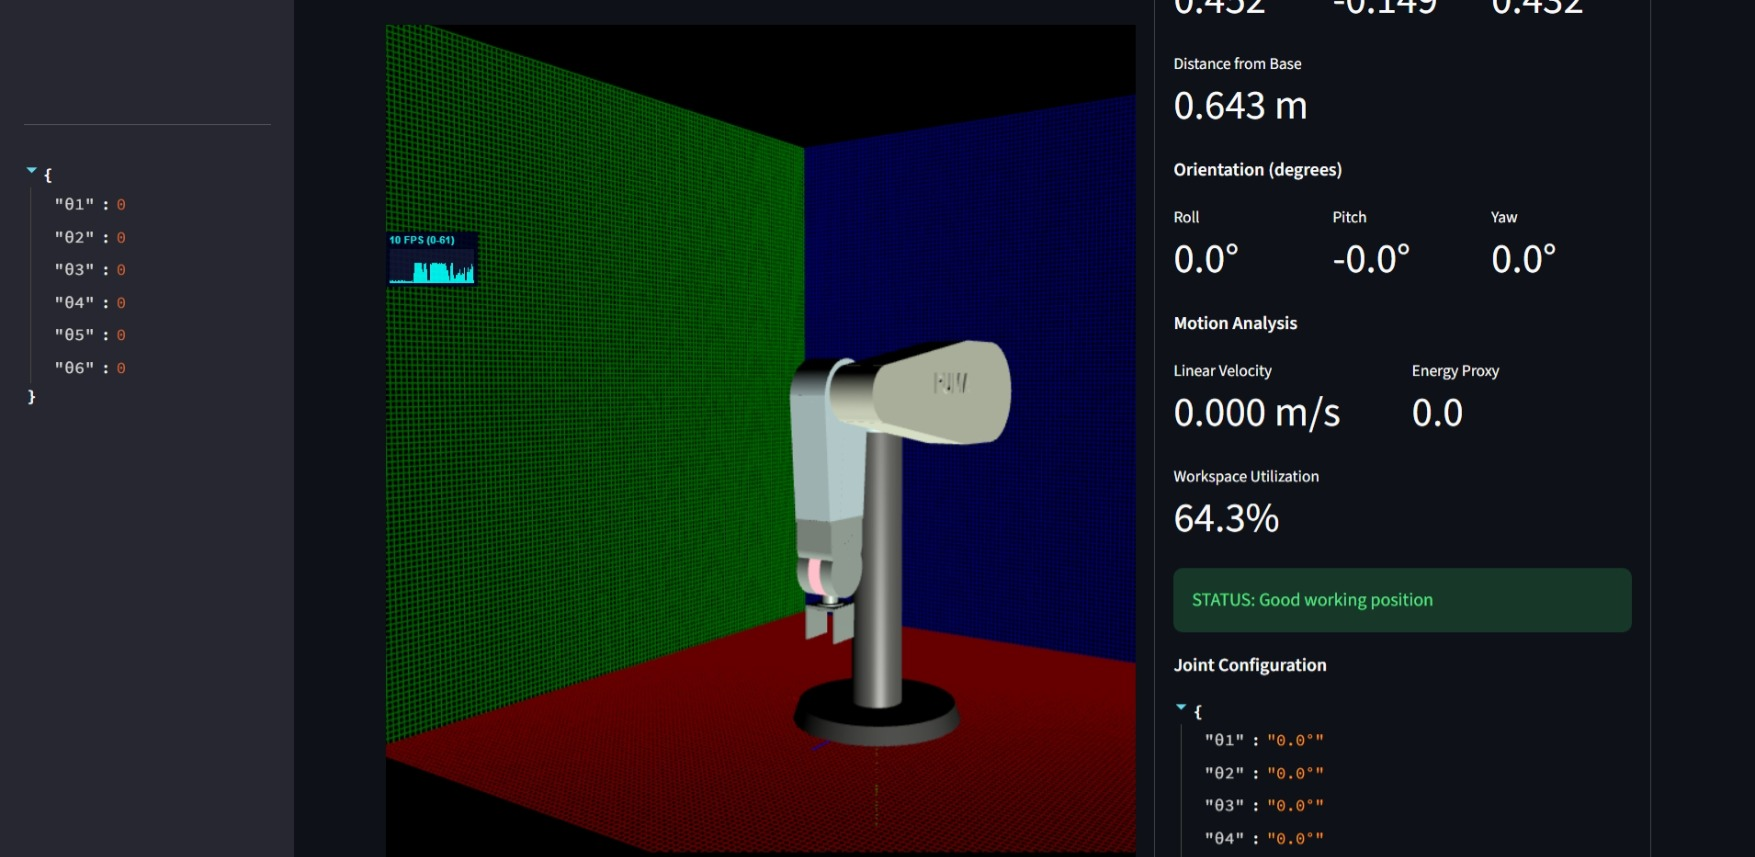
\includegraphics[width=3.5in]{images/main_ui.jpeg}
\caption{The main user interface of the PUMA 560 Digital Twin showing the complete Streamlit-based interface with professional branding, performance indicators (1.7ms render time), trajectory recording controls, comprehensive joint control sliders for all six degrees of freedom, and the End-Effector Analytics panel displaying real-time position coordinates. The interface demonstrates the integration with IIT KGP Virtual Labs and includes optimization features like lazy loading and cached assets.}
\label{fig:main_ui}
\end{figure}

\begin{table}[!t]
\renewcommand{\arraystretch}{1.3}
\caption{Denavit-Hartenberg Parameters for the PUMA 560}
\label{tab:dh_parameters}
\centering
\begin{tabular}{|c|c|c|c|c|}
\hline
\textbf{Joint (i)} & \textbf{$\theta_i$ (rad)} & \textbf{$d_i$ (m)} & \textbf{$a_i$ (m)} & \textbf{$\alpha_i$ (rad)} \\
\hline
1 & $\theta_1$ & 0.0 & 0.0 & $\pi/2$ \\
\hline
2 & $\theta_2$ & 0.0 & 0.432 & 0.0 \\
\hline
3 & $\theta_3$ & 0.1495 & 0.0203 & $-\pi/2$ \\
\hline
4 & $\theta_4$ & 0.432 & 0.0 & $\pi/2$ \\
\hline
5 & $\theta_5$ & 0.0 & 0.0 & $-\pi/2$ \\
\hline
6 & $\theta_6$ & 0.0 & 0.0 & 0.0 \\
\hline
\end{tabular}
\end{table}

\subsection{Real-Time Kinematic Analysis}
As users adjust the joint angles, the backend continuously recalculates the robot's state. The DH parameters, as listed in Table~\ref{tab:dh_parameters}, are used to compute the transformation matrix for each link. The detailed analytics interface (Fig.~\ref{fig:detailed_analytics}) provides comprehensive real-time feedback.



The comprehensive real-time analytics interface provides immediate feedback on all aspects of the robot's current state. The system displays precise end-effector position coordinates, distance from base, complete orientation analysis (Roll, Pitch, Yaw), motion analysis including linear velocity and energy consumption proxy, workspace utilization percentage, and an intelligent status indicator that provides operational feedback ("Good working position", singularity warnings, etc.). All joint angles are displayed in real-time with high precision, and the system maintains smooth performance monitoring with frame rate indicators.

\begin{figure}[!t]
\centering
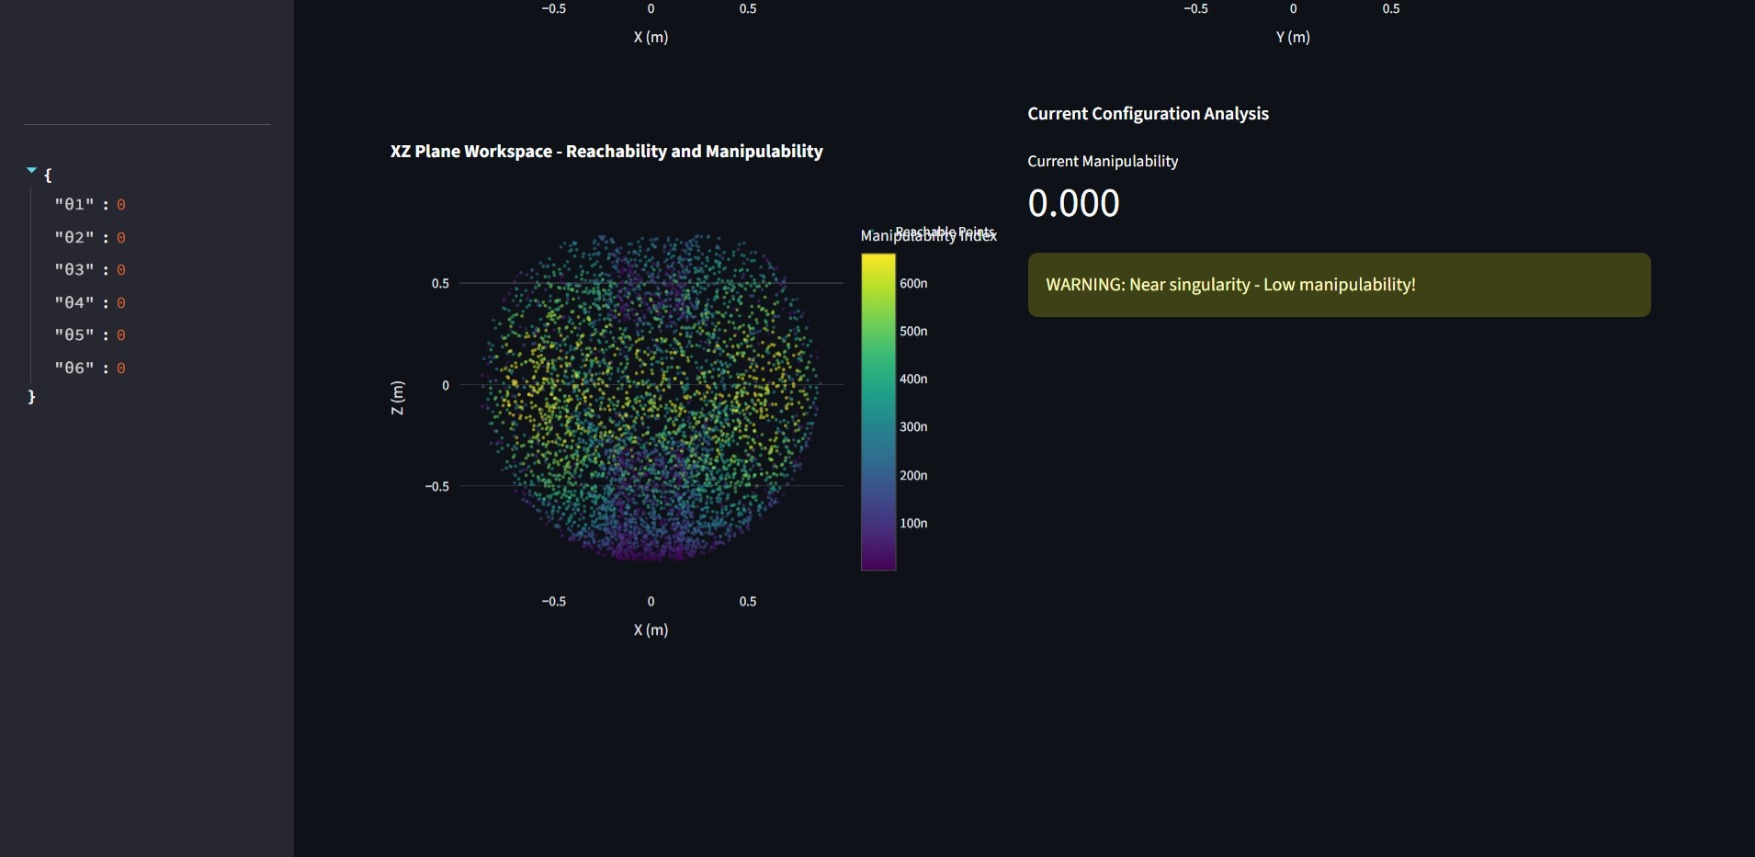
\includegraphics[width=3.5in]{images/detailed_ui.jpeg}
\caption{Complete interface showing the 3D PUMA 560 robot model with coordinate grid and comprehensive real-time analytics panel. The analytics display end-effector position coordinates (0.432, -0.149, 0.432), distance from base (0.643 m), orientation angles (Roll, Pitch, Yaw), motion analysis with linear velocity and energy proxy, workspace utilization (64.3\%), operational status indicator, and complete joint configuration data.}
\label{fig:detailed_analytics}
\end{figure}

\subsection{Trajectory Recording and Visualization}
The system includes a full trajectory analysis suite. Users can start and stop recording, and the application will store a list of state dictionaries. When the recording is complete, the data is loaded into a Pandas DataFrame and visualized using Plotly within a set of \texttt{st.tabs}, as shown in Fig.~\ref{fig:trajectory_analysis}. Advanced energy analysis capabilities (Fig.~\ref{fig:energy_analysis}) provide additional insights into motion dynamics. The following plots are generated:

\begin{figure}[!t]
\centering
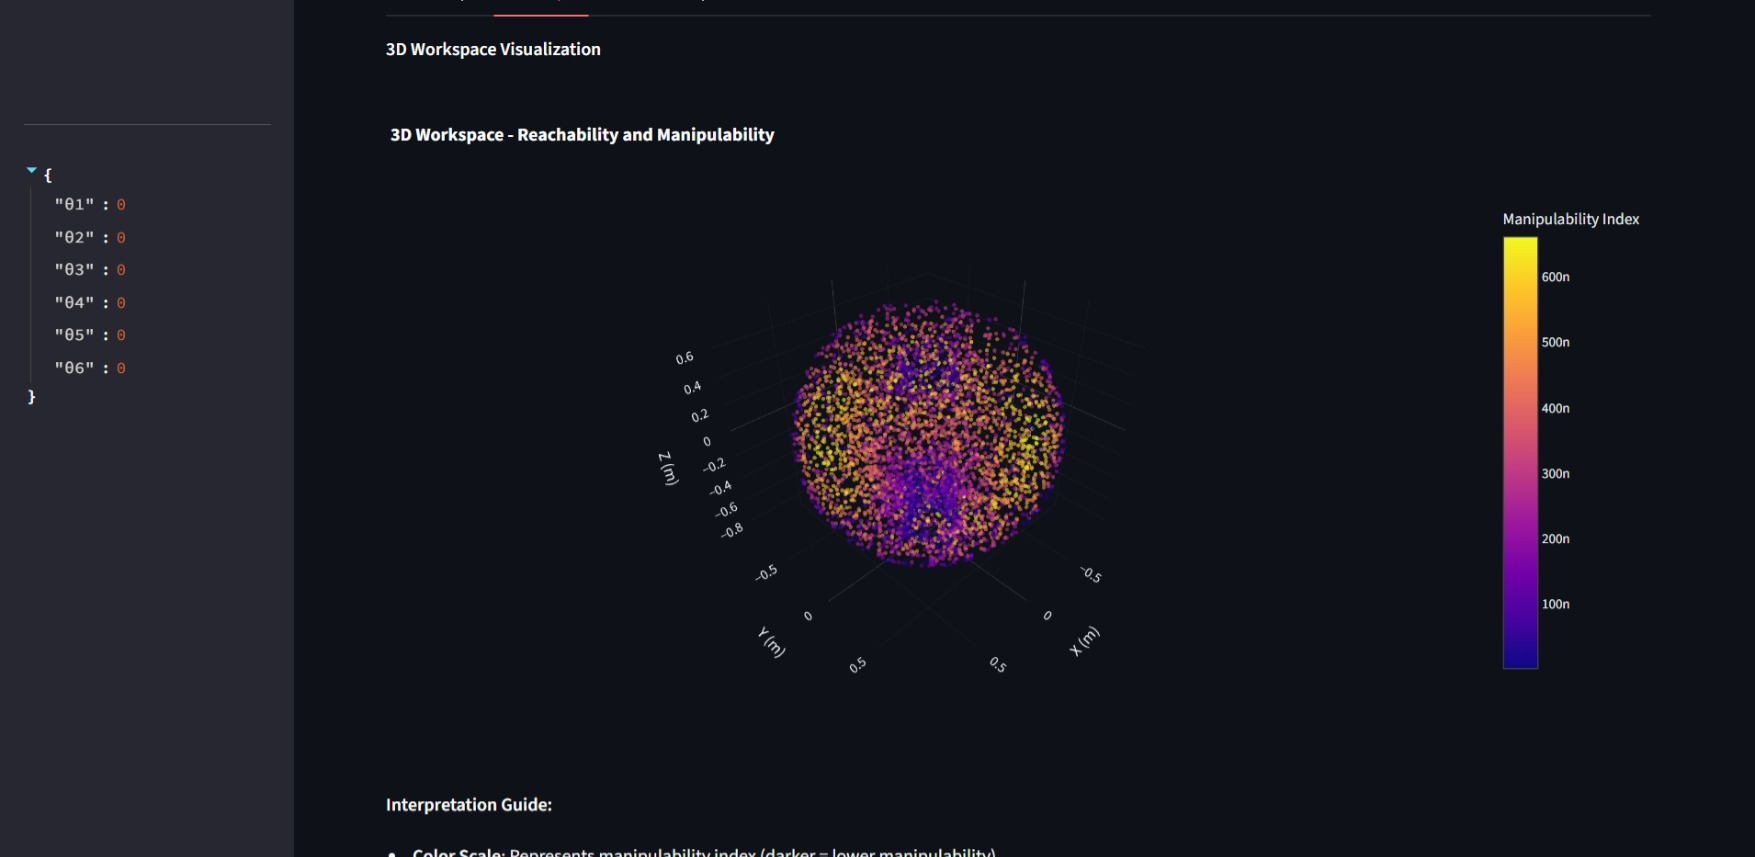
\includegraphics[width=3.5in]{images/trajectory_ui.jpeg}
\caption{The Trajectory Analysis section showing the multi-tabbed interface with Plotly visualizations for joint angles over time, 3D end-effector path tracking, velocity analysis, and data export capabilities with CSV download functionality.}
\label{fig:trajectory_analysis}
\end{figure}

The trajectory visualization system generates multiple analytical perspectives of the recorded motion data. A comprehensive timeline displays the angular position of all six joints throughout the recorded sequence, enabling students to observe coordination patterns and joint coupling effects. Additionally, a three-dimensional scatter plot renders the end-effector's spatial path through the workspace, providing intuitive visualization of the tool's movement trajectory. The system also generates detailed timelines of joint velocities and end-effector linear velocity, facilitating analysis of motion smoothness and dynamic characteristics. All captured trajectory data can be exported to CSV format with a single click, enabling further analysis in external software tools or integration with laboratory reports.

\begin{figure}[!t]
\centering
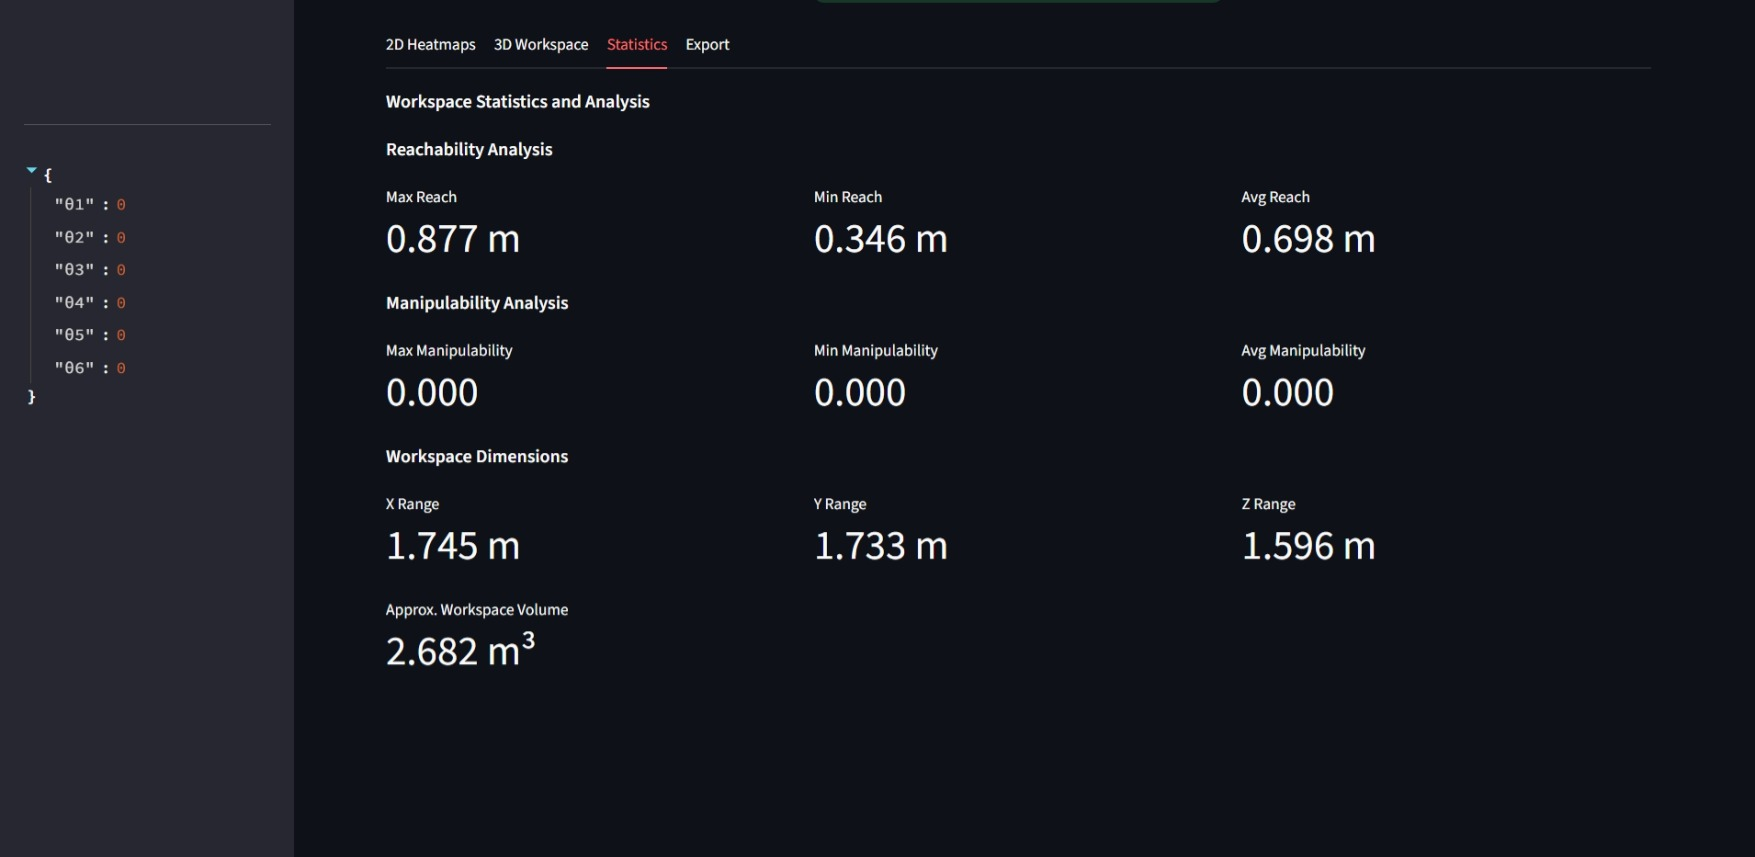
\includegraphics[width=3.5in]{images/energy_ui.jpeg}
\caption{Advanced trajectory analysis showing energy consumption calculations, joint velocity profiles, and motion dynamics. The interface demonstrates comprehensive kinematic and dynamic analysis capabilities for educational robotics applications.}
\label{fig:energy_analysis}
\end{figure}

\subsection{Workspace Analysis and Manipulability}
The system provides comprehensive workspace analysis through 2D manipulability heatmaps, 3D visualizations, and real-time singularity detection. Using Monte Carlo sampling with up to 20,000 random joint configurations, the platform generates detailed 2D heatmap projections across different coordinate planes (XY, XZ, YZ) as shown in Fig.~\ref{fig:workspace_heatmaps}. The 2D heatmap visualization displays color-coded manipulability indices ranging from 100n to 600n, where warmer colors (yellow-green) indicate regions of higher dexterity and cooler colors (blue-purple) represent areas with reduced manipulability. The interface includes real-time current configuration analysis with automatic singularity detection, providing immediate feedback when the robot approaches configurations with low manipulability through prominent warning notifications.

\begin{figure}[!t]
\centering
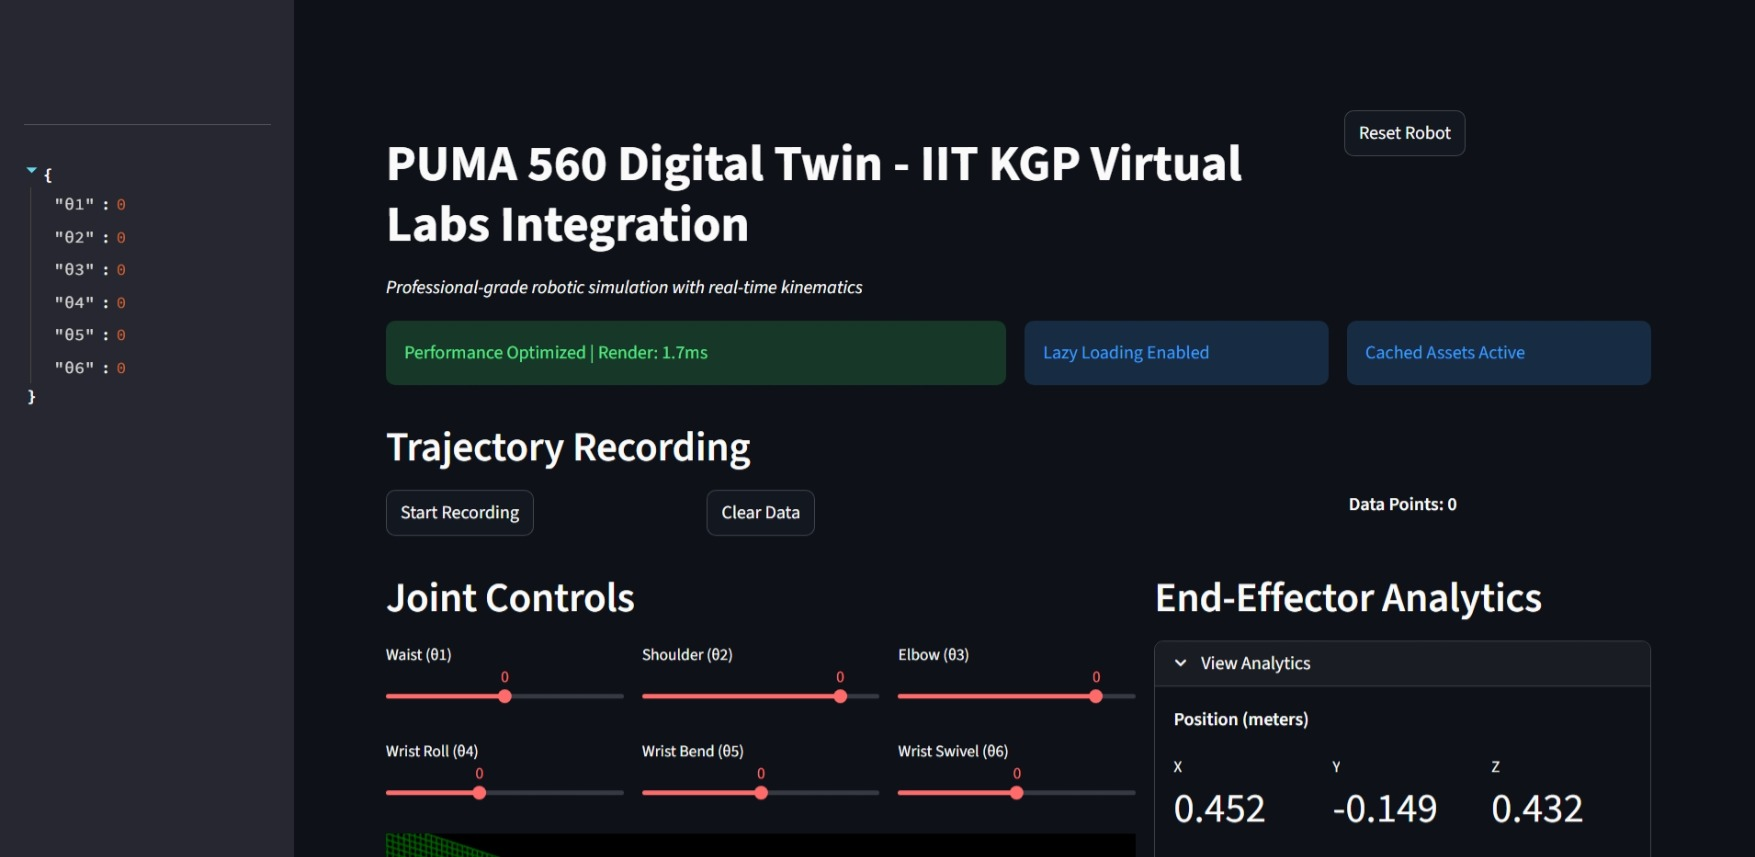
\includegraphics[width=3.5in]{images/workspace_ui.jpeg}
\caption{2D Heatmap workspace analysis showing the XZ plane reachability and manipulability visualization. The color-coded heatmap displays manipulability index values from 100n to 600n across the X-Z coordinate space, with the current configuration analysis panel showing real-time manipulability assessment. The interface demonstrates singularity detection capabilities with a warning system for low manipularity regions.}
\label{fig:workspace_heatmaps}
\end{figure}

The manipulability index, computed from the Jacobian matrix determinant, provides insight into the robot's dexterity at different configurations. The system continuously monitors the current robot configuration and displays real-time manipulability values, automatically generating warning notifications when approaching singularity conditions (manipulability $\approx$ 0.000). Low manipulability regions indicate potential singularities where the robot loses degrees of freedom, while high manipulability areas represent optimal working zones for precise manipulation tasks.

\begin{figure}[!t]
\centering
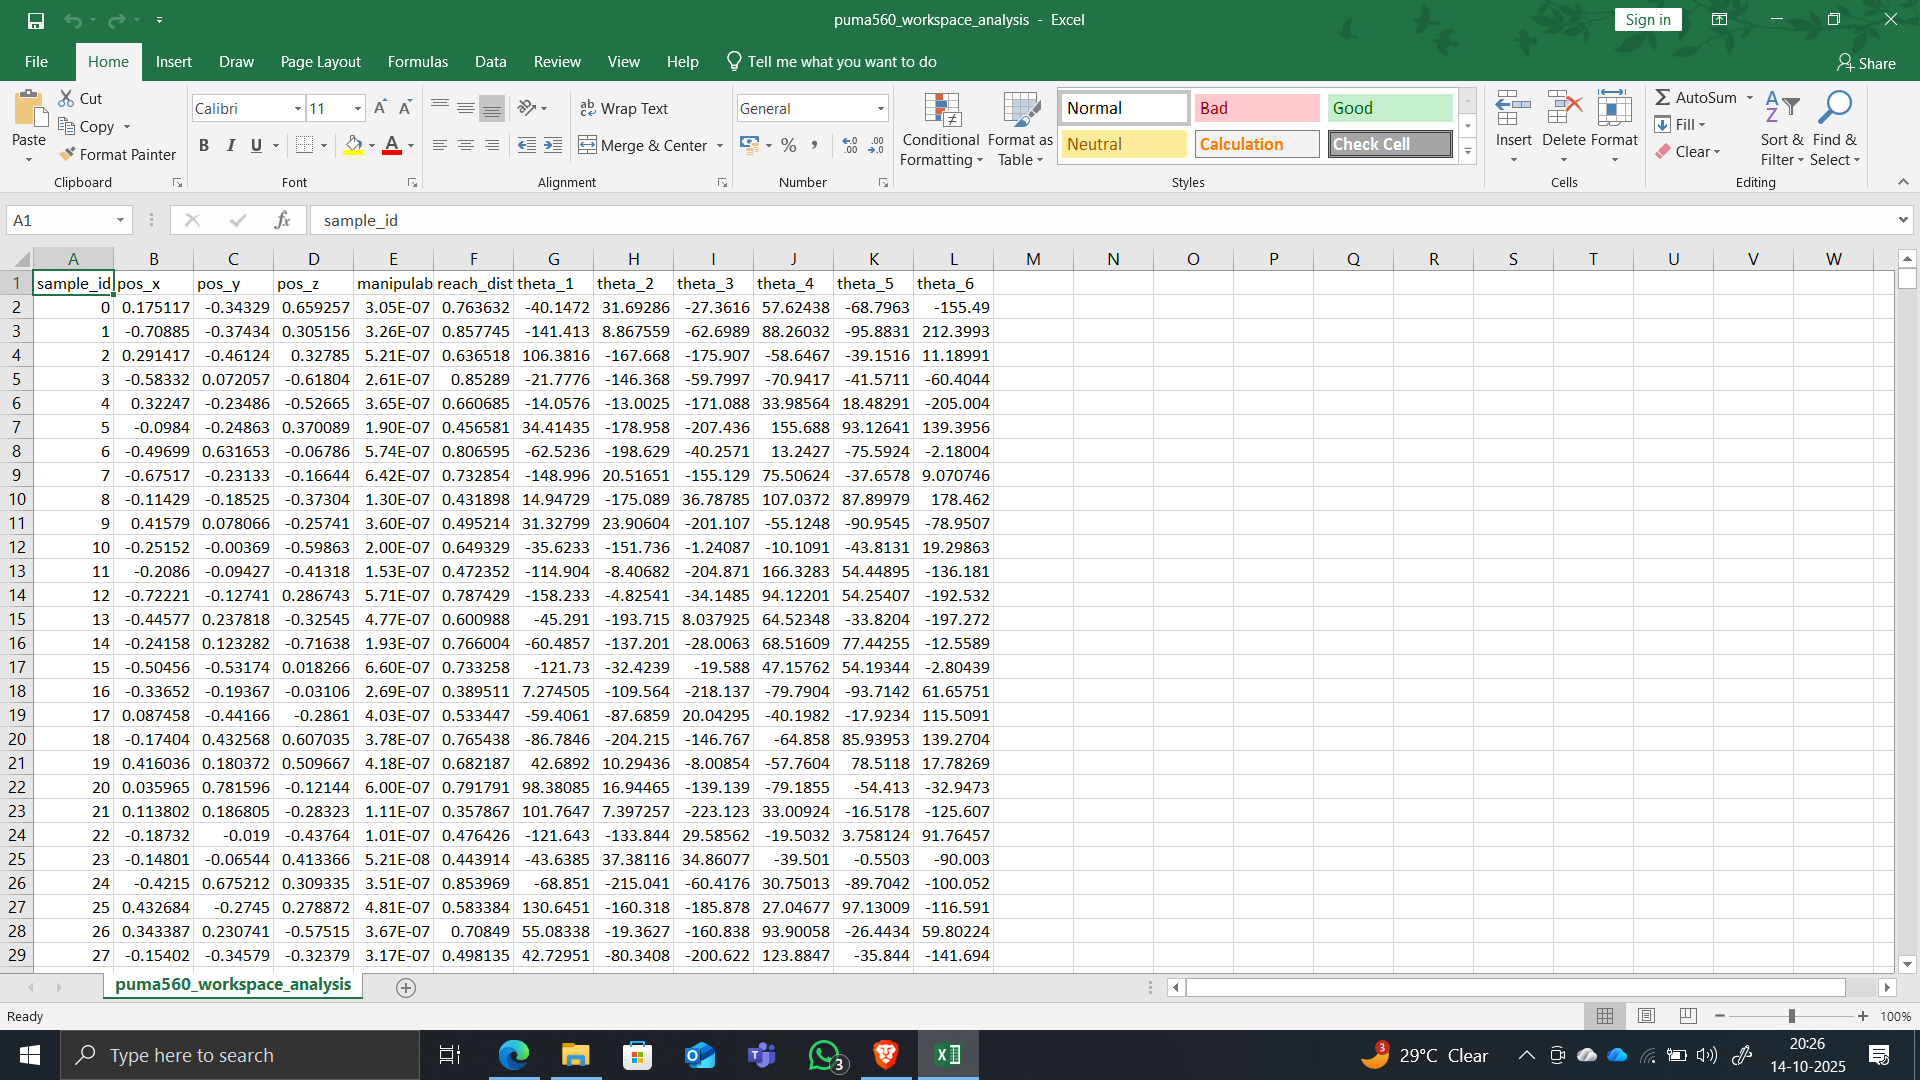
\includegraphics[width=3.5in]{images/image.png}
\caption{Complete system overview demonstrating the integrated platform with simultaneous 3D visualization, real-time analytics, trajectory recording, and workspace analysis capabilities. This comprehensive interface showcases the full potential of the modernized PUMA 560 digital twin for robotics education.}
\label{fig:system_overview}
\end{figure}

\section{Conclusion}
This project successfully demonstrates the creation of a modern, web-based digital twin for the PUMA 560 robot. By leveraging a Python-centric stack with Streamlit and integrating a JavaScript-based 3D renderer, we have produced a tool that is both powerful for analysis and simple to access. The complete integrated system (Fig.~\ref{fig:system_overview}) showcases the seamless integration of all components. The modular architecture and detailed, real-time analytics provide a robust foundation for robotics education. Future work could include the implementation of inverse kinematics to allow for Cartesian control, the integration of PyBullet for physics-based simulation and collision detection, and the development of more advanced workspace analysis tools.

\section*{Acknowledgment}
The authors acknowledge the foundational work of the IIT Kharagpur Virtual Labs project. The Three.js 3D model and its original JavaScript implementation were adapted from their ”Forward Kinematics of PUMA 560” experiment, which provided the core assets and inspiration for this modern re-implementation.

\begin{thebibliography}{00}
\bibitem{b1} R. P. Paul, B. Shimano, and G. E. Mayer, ``Kinematic control equations for simple manipulators,'' \emph{IEEE Transactions on Systems, Man, and Cybernetics}, vol. 11, no. 6, pp. 449-455, 1981.
\bibitem{b2} J. J. Craig, \emph{Introduction to Robotics: Mechanics and Control}, 3rd ed. Pearson/Prentice Hall, 2005.
\bibitem{b3} Streamlit Inc., ``Streamlit: The fastest way to build and share data apps,'' 2024. [Online]. Available: https://streamlit.io
\bibitem{b4} Mr.doob, ``Three.js: JavaScript 3D library,'' 2024. [Online]. Available: https://threejs.org
\bibitem{b5} E. Coumans and Y. Bai, ``PyBullet, a Python module for physics simulation for games, robotics and machine learning,'' 2016-2021. [Online]. Available: http://pybullet.org
\bibitem{b6} J. D. Hunter, ``Matplotlib: A 2D graphics environment,'' \emph{Computing in Science \& Engineering}, vol. 9, no. 3, pp. 90-95, 2007.
\bibitem{b7} Plotly Technologies Inc., ``Collaborative data science,'' 2015. [Online]. Available: https://plot.ly.
\end{thebibliography}

\end{document}
